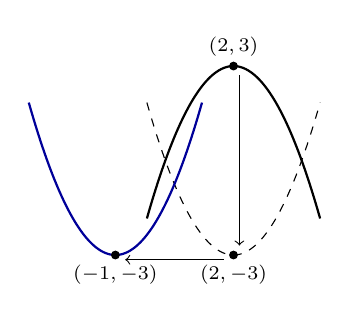
\begin{tikzpicture}[x=5mm,y=4mm]
\ax{-4}{5}{-4.5}{4.5}
\draw[thick,domain=-0.2:4.2,samples=80] plot (\x,{-(\x-2)^2+3});
\draw[dashed,domain=-0.2:4.2,samples=80] plot (\x,{(\x-2)^2-3});
\draw[thick,blue!60!black,domain=-3.2:1.2,samples=80] plot (\x,{(\x+1)^2-3});
\fill (2,3) circle (1.6pt);
\node[above] at (2,3){\scriptsize $(2,3)$};
\fill (2,-3) circle (1.6pt);
\node[below] at (2,-3){\scriptsize $(2,-3)$};
\fill (-1,-3) circle (1.6pt);
\node[below] at (-1,-3){\scriptsize $(-1,-3)$};
\draw[->] (2.15,2.7)--(2.15,-2.7); \draw[->] (1.75,-3.15)--(-0.75,-3.15);
\end{tikzpicture}